\documentclass[aspectratio=169]{beamer}
\usepackage[T1]{fontenc}
\usepackage[utf8]{inputenc}
\usepackage{lmodern}
\usepackage{microtype}
\usepackage{xcolor}
\usepackage{tikz}
\usetikzlibrary{positioning, arrows.meta, calc}
\usepackage{fontawesome5}
\definecolor{wurgreen}{HTML}{34B233}
\definecolor{darkgreen}{HTML}{1F6B1E}
\definecolor{darknavy}{HTML}{1A1A2E}
\definecolor{midgray}{HTML}{6B7280}
\definecolor{lightgray}{HTML}{F3F4F6}
\definecolor{lightgreen}{HTML}{E8F7E8}
\definecolor{bodytext}{HTML}{1F2937}
\definecolor{warnred}{HTML}{FEE2E2}
\definecolor{warnborder}{HTML}{EF4444}
\definecolor{codebg}{HTML}{1E1E2E}
\definecolor{codegreen}{HTML}{9ECE6A}
\definecolor{codeblue}{HTML}{7AA2F7}
\definecolor{codeorange}{HTML}{FF9E64}
\definecolor{codegray}{HTML}{C0CAF5}
\usetheme{default}\usecolortheme{default}\usefonttheme{professionalfonts}
\setbeamertemplate{navigation symbols}{}
\setbeamertemplate{itemize items}{\textcolor{wurgreen}{\textbullet}}
\setbeamertemplate{itemize subitem}{\textcolor{midgray}{--}}
\setbeamercolor{frametitle}{fg=white, bg=darknavy}
\setbeamerfont{frametitle}{size=\large, series=\bfseries}
\setbeamertemplate{frametitle}{%
  \begin{beamercolorbox}[wd=\paperwidth, ht=1.1cm, dp=0.2cm, leftskip=0.6cm]{frametitle}
    \usebeamerfont{frametitle}\insertframetitle\end{beamercolorbox}}
\setbeamercolor{background canvas}{bg=white}
\setbeamercolor{normal text}{fg=bodytext}
\setbeamertemplate{footline}{%
  \begin{beamercolorbox}[wd=\paperwidth, ht=0.4cm, dp=0.15cm]{footline}
    \hspace{0.5cm}\textcolor{midgray}{\tiny Introduction to Python · Module 3: Control Flow}%
    \hfill\textcolor{midgray}{\tiny \insertframenumber}\hspace{0.4cm}\end{beamercolorbox}}
\newcommand{\codebox}[1]{\begin{center}
  \begin{tikzpicture}\node[fill=codebg, rounded corners=4pt, inner sep=9pt, text width=0.85\textwidth, text=codegray]{\ttfamily\small #1};\end{tikzpicture}\end{center}}
\begin{document}
{\setbeamertemplate{footline}{}
\begin{frame}[plain]
  \begin{tikzpicture}[remember picture, overlay]
    \fill[darknavy] (current page.south west) rectangle (current page.north east);
    \fill[wurgreen] (current page.south west) rectangle ([xshift=0.45cm]current page.north west);
    \node[anchor=west, text=white, font=\huge\bfseries, text width=13cm] at ([xshift=1.1cm, yshift=1.4cm]current page.west){Introduction to Python};
    \node[anchor=west, text=wurgreen, font=\large, text width=12cm] at ([xshift=1.1cm, yshift=0.2cm]current page.west){Module 3 --- Control Flow};
    \node[anchor=west, text=midgray, font=\small, text width=12cm] at ([xshift=1.1cm, yshift=-1.3cm]current page.west){Conditionals and loops};
  \end{tikzpicture}
\end{frame}}

\begin{frame}{Making Decisions: \texttt{if}}
\vspace{0.2cm}
{\small Programs need to \textbf{react} to different situations. The \texttt{if} statement runs
code only when a condition is \texttt{True}.}
\medskip
\codebox{%
score \textcolor{codegray}{=} \textcolor{codeorange}{72}\\[6pt]
\textcolor{codeblue}{if} score \textcolor{codegray}{>=} \textcolor{codeorange}{60}:\\
\quad\textcolor{codeblue}{print}(\textcolor{codegreen}{"Pass"})\\
\textcolor{codeblue}{else}:\\
\quad\textcolor{codeblue}{print}(\textcolor{codegreen}{"Fail"})}
\medskip
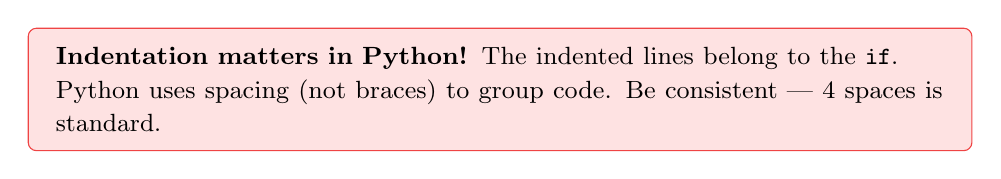
\begin{tikzpicture}
  \node[fill=warnred, draw=warnborder, rounded corners=3pt, inner xsep=10pt, inner ysep=7pt, text width=\textwidth-24pt]{%
    {\small \textbf{Indentation matters in Python!} The indented lines belong to the \texttt{if}.
    Python uses spacing (not braces) to group code. Be consistent --- 4 spaces is standard.}};
\end{tikzpicture}
\end{frame}

\begin{frame}{More Conditions: \texttt{elif} and Comparisons}
\vspace{0.2cm}
{\small Chain multiple conditions with \texttt{elif} (``else if''). Python checks them in order
and runs the \emph{first} match.}
\medskip
\codebox{%
\textcolor{codeblue}{if} score \textcolor{codegray}{>=} \textcolor{codeorange}{85}:\\
\quad grade \textcolor{codegray}{=} \textcolor{codegreen}{"A"}\\
\textcolor{codeblue}{elif} score \textcolor{codegray}{>=} \textcolor{codeorange}{70}:\\
\quad grade \textcolor{codegray}{=} \textcolor{codegreen}{"B"}\\
\textcolor{codeblue}{else}:\\
\quad grade \textcolor{codegray}{=} \textcolor{codegreen}{"C"}}
\medskip
{\small The \textbf{comparison operators}: \texttt{==} (equal), \texttt{!=} (not equal),
\texttt{<}, \texttt{>}, \texttt{<=}, \texttt{>=}. Combine conditions with \texttt{and},
\texttt{or}, \texttt{not}.}
\medskip
{\small\textcolor{midgray}{\textit{Careful: \texttt{=} assigns a value, \texttt{==} \emph{tests}
for equality. Mixing them up is a classic bug.}}}
\end{frame}

\begin{frame}{Repeating: \texttt{for} Loops}
\vspace{0.2cm}
{\small A \texttt{for} loop runs a block of code \textbf{once for each item} in a collection.
This is how you process every document, word, or row.}
\medskip
\codebox{%
words \textcolor{codegray}{=} [\textcolor{codegreen}{"cat"}, \textcolor{codegreen}{"dog"}, \textcolor{codegreen}{"bird"}]\\[6pt]
\textcolor{codeblue}{for} word \textcolor{codeblue}{in} words:\\
\quad\textcolor{codeblue}{print}(word.\textcolor{codeblue}{upper}())\\[6pt]
\textcolor{codegray}{\# CAT}\\
\textcolor{codegray}{\# DOG}\\
\textcolor{codegray}{\# BIRD}}
\medskip
{\small The variable \texttt{word} takes each value in turn. The indented body runs once per
item. This is the single most common pattern in data work.}
\end{frame}

\begin{frame}{Looping Tools: \texttt{range} and \texttt{enumerate}}
\vspace{0.2cm}
\begin{columns}[T]
  \column{0.5\textwidth}\vspace{0pt}
  {\small\textbf{\texttt{range(n)}} --- loop a fixed number of times:}
  \smallskip
  \codebox{%
  \textcolor{codeblue}{for} i \textcolor{codeblue}{in} \textcolor{codeblue}{range}(\textcolor{codeorange}{3}):\\
  \quad\textcolor{codeblue}{print}(i)\\
  \textcolor{codegray}{\# 0}\\
  \textcolor{codegray}{\# 1}\\
  \textcolor{codegray}{\# 2}}
  \column{0.5\textwidth}\vspace{0pt}
  {\small\textbf{\texttt{enumerate()}} --- get position \emph{and} item:}
  \smallskip
  \codebox{%
  \textcolor{codeblue}{for} i, w \textcolor{codeblue}{in} \textcolor{codeblue}{enumerate}(words):\\
  \quad\textcolor{codeblue}{print}(i, w)\\
  \textcolor{codegray}{\# 0 cat}\\
  \textcolor{codegray}{\# 1 dog}\\
  \textcolor{codegray}{\# 2 bird}}
\end{columns}
\medskip
{\small\textcolor{midgray}{\textit{There's also the \texttt{while} loop, which repeats \emph{as
long as} a condition holds --- useful, but \texttt{for} covers most needs.}}}
\end{frame}

\begin{frame}{A Complete Example: Counting Words}
\vspace{0.2cm}
{\small Putting it together --- loops, conditions, and a dictionary to count words:}
\medskip
\codebox{%
text \textcolor{codegray}{=} [\textcolor{codegreen}{"cat"}, \textcolor{codegreen}{"dog"}, \textcolor{codegreen}{"cat"}, \textcolor{codegreen}{"bird"}, \textcolor{codegreen}{"cat"}]\\
counts \textcolor{codegray}{=} \{\}\\[6pt]
\textcolor{codeblue}{for} word \textcolor{codeblue}{in} text:\\
\quad\textcolor{codeblue}{if} word \textcolor{codeblue}{in} counts:\\
\quad\quad counts[word] \textcolor{codegray}{+=} \textcolor{codeorange}{1}\\
\quad\textcolor{codeblue}{else}:\\
\quad\quad counts[word] \textcolor{codegray}{=} \textcolor{codeorange}{1}\\[6pt]
\textcolor{codegray}{\# counts is now \{"cat": 3, "dog": 1, "bird": 1\}}}
\medskip
{\small\textcolor{midgray}{\textit{This is essentially what a word-frequency counter does ---
you built one from scratch!}}}
\end{frame}

\begin{frame}{Module 3: Takeaways}
\vspace{0.3cm}
\begin{itemize}\setlength\itemsep{8pt}
  \item[\textcolor{wurgreen}{\faCheck}] \texttt{if} / \texttt{elif} / \texttt{else} run code based on \textbf{conditions}
  \item[\textcolor{wurgreen}{\faCheck}] \textbf{Indentation} defines what belongs to a block --- be consistent
  \item[\textcolor{wurgreen}{\faCheck}] Compare with \texttt{== != < > <= >=}; combine with \texttt{and or not}
  \item[\textcolor{wurgreen}{\faCheck}] \texttt{for ... in} loops over every item in a collection
  \item[\textcolor{wurgreen}{\faCheck}] \texttt{range()} and \texttt{enumerate()} are your looping companions
\end{itemize}
\medskip
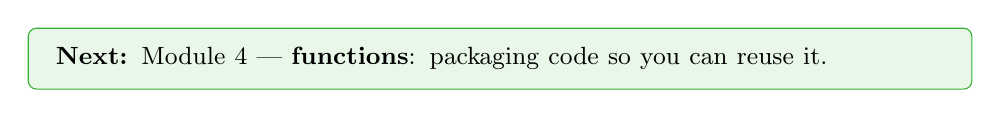
\begin{tikzpicture}
  \node[fill=lightgreen, draw=wurgreen, rounded corners=3pt, inner xsep=10pt, inner ysep=7pt, text width=\textwidth-24pt]{%
    {\small \textbf{Next:} Module 4 --- \textbf{functions}: packaging code so you can reuse it.}};
\end{tikzpicture}
\end{frame}
\end{document}
